\section{SIMULATION RESULTS}

\subsection{BLOCK DIAGRAM OF THE SYSTEM}



The block diagram of the Field-Oriented Control (FOC) system for an AC induction motor is shown in Figure \ref{fig:block_diagram}. The system consists of two main subsystems: the Speed Control Subsystem and the Current Control Subsystem. The Speed Control Subsystem is responsible for generating the torque reference values based on the speed reference and feedback values. The Current Control Subsystem is responsible for tracking the reference currents and generating the appropriate voltage references for the inverter to control the motor's currents. The system also includes a Current Measurement block, a Flux Observer block, and a Speed Estimation block to provide the necessary feedback signals for the control system.


The current control system is a run on ADC end of converion interrupt. The system operates at a PWM frequency of 15 kHz.

\begin{figure}[H]
	\centering
	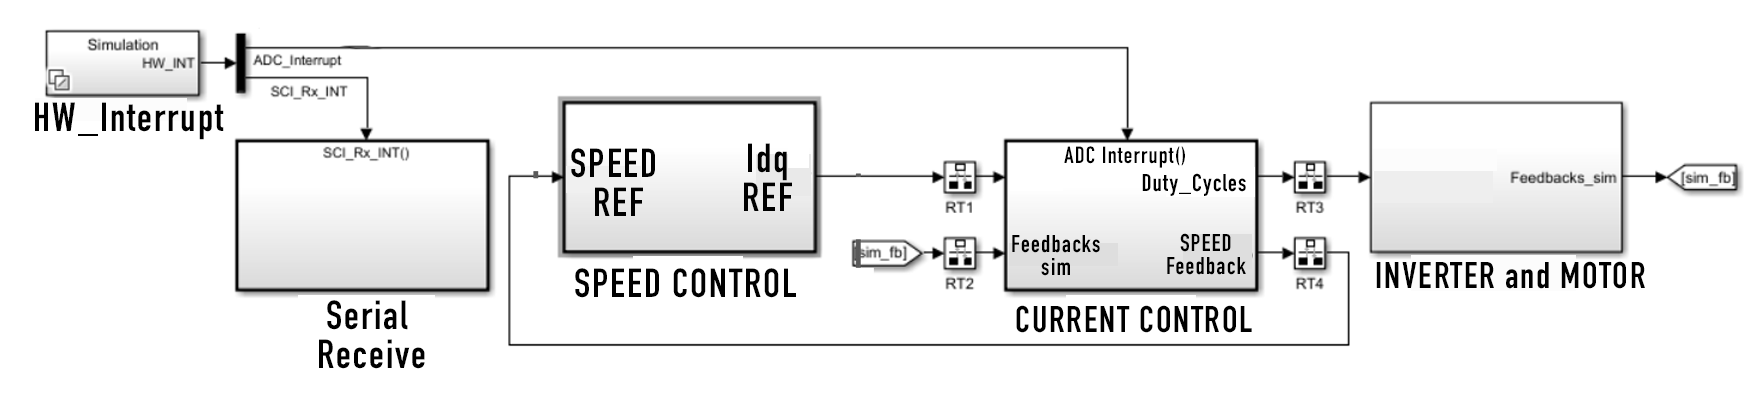
\includegraphics[width=6in]{sections/section3/images/simulation/blockDia.png}
	\caption{Block Diagram of the System}
	\label{fig:block_diagram}
\end{figure}


\subsection{SOFTWARE FLOW CHART}

\begin{figure}[H]
	\centering
	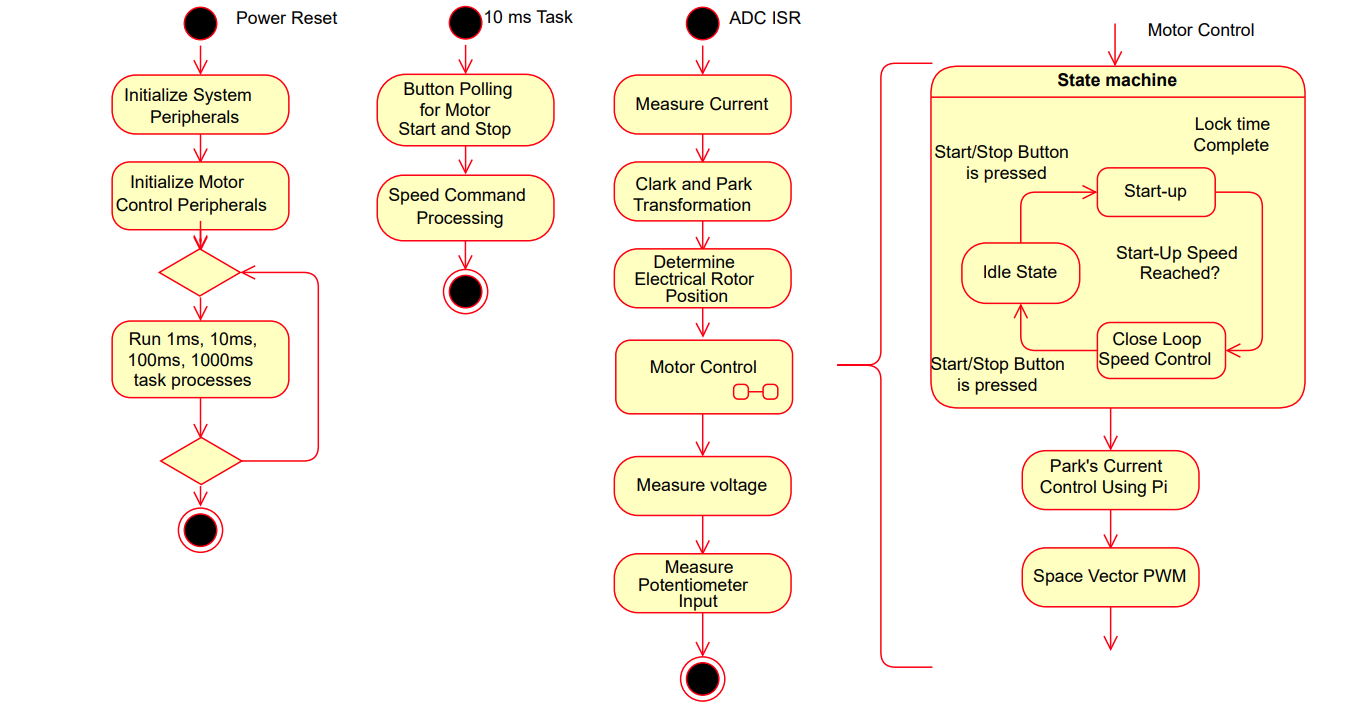
\includegraphics[width=6in]{sections/section3/images/softwareflowchart.png}
	\caption{Software Flow Chart}
	\label{fig:Software Flow Chart}
\end{figure}

The software flow chart in Figure \ref{fig:Software Flow Chart} illustrates the sequence of operations in the FOC control system for an AC induction motor. The flow chart outlines the key steps involved in the control process, including the initialization of the system, the measurement of the motor's currents and voltages, the estimation of the motor's speed and position, and the generation of the appropriate control signals to regulate the motor's speed and torque.


\subsection{SPEED CONTROL SUBSYSTEM}

The speed control system shown in Figure \ref{fig:speed_control_system} consists of a DataStoreRead block that holds the speed reference value received from the host computer, a Discrete IIR lowpass filter block to cancel the zeros in the system, and a Discrete PID Controller with anti-windup block that takes the speed reference and feedback values as inputs and generates the torque reference as output. 

\begin{figure}[H]
	\centering
	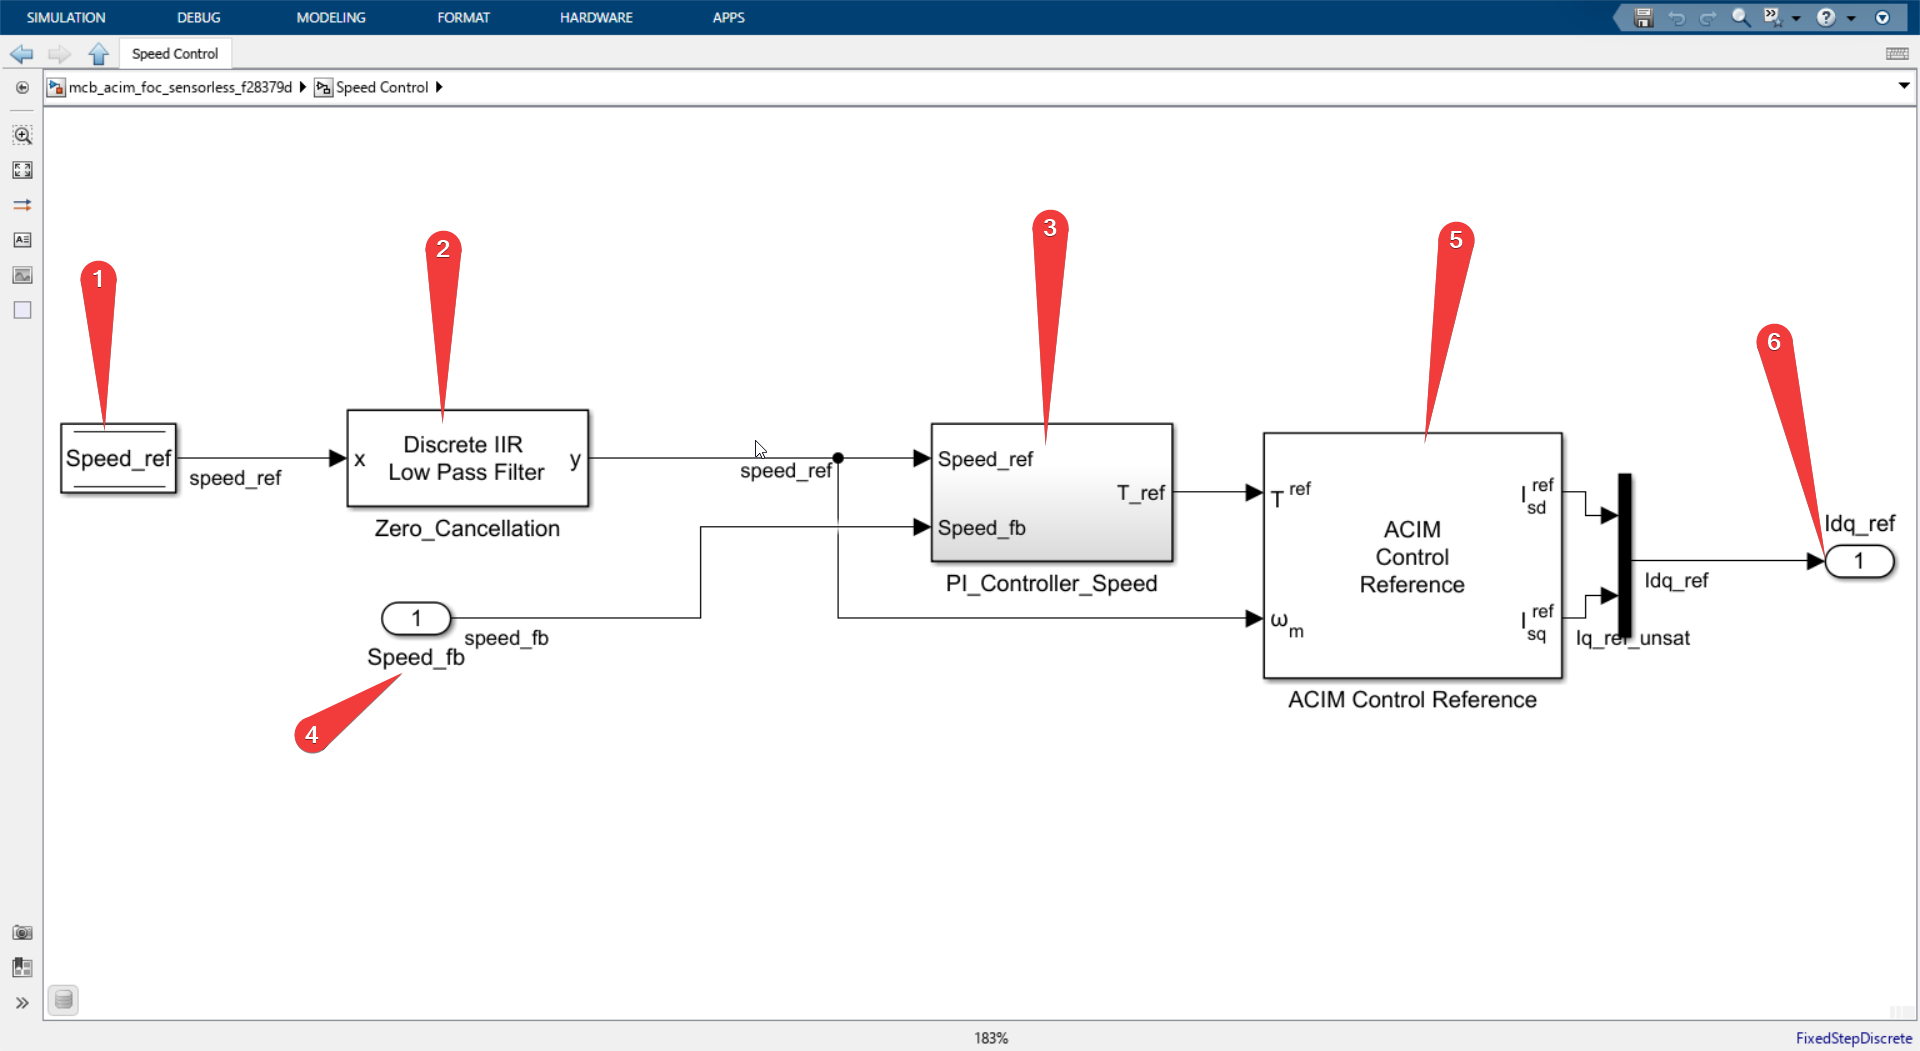
\includegraphics[width=5in]{sections/section3/images/simulation/speedControl/speedController.png}
	\caption{Speed Control System}
	\label{fig:speed_control_system}
\end{figure}


The ACIM Control reference block then takes the torque reference and speed reference as inputs and generates the $Isd_{ref}$ and $Isq_{ref}$ values, which are the reference values for the current control loop. The DQ limiter block is used to limit the magnitude of the vector represented in the d-q reference frame, with the option to prioritize either the d-axis or q-axis component.


\subsection{CURRENT CONTROL SUBSYSTEM}


\subsubsection{Current Measurement}


The current measurement part of the Input Scaling block shown in Figure \ref{fig:current_measurement}

\begin{figure}[H]
	\centering
	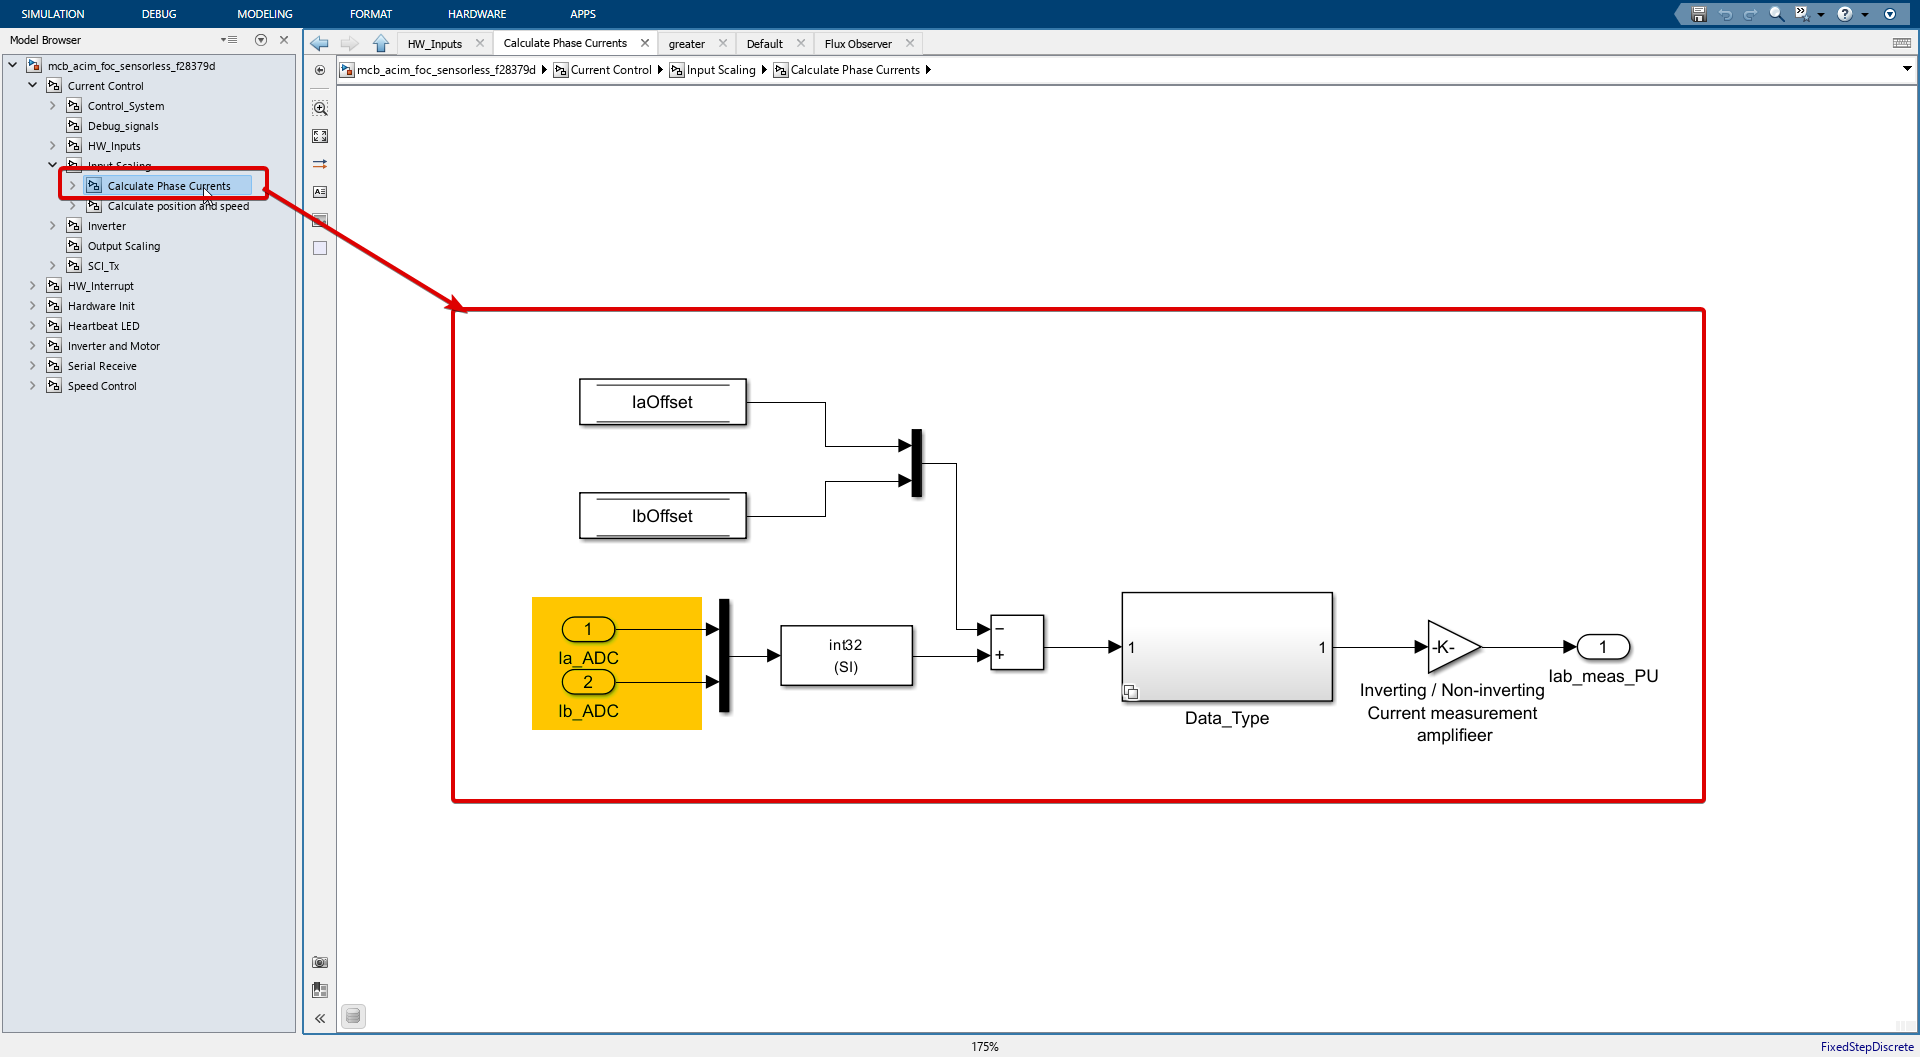
\includegraphics[width=4in]{sections/section3/images/simulation/inputScaling/currentMeasurement.png}
	\caption{Current Measurement}
	\label{fig:current_measurement}
\end{figure}


converts the $Ia_{ADC}$ and $Ib_{ADC}$ inputs from the ADCs to the appropriate data type (int32) and removes the offsets ($Ia_{offset}$ and $Ib_{offset}$) that were previously calibrated. The signals then go through a series of gain blocks to convert them to per-unit (PU) values. The first gain block converts the ADC voltage to the actual voltage, the second gain block converts the voltage to current using the inverter's current sense voltage per amp, and the third gain block converts the current to PU using the motor's base current.


\subsubsection{Position And Speed Estimation}



\begin{figure}[H]
	\centering
	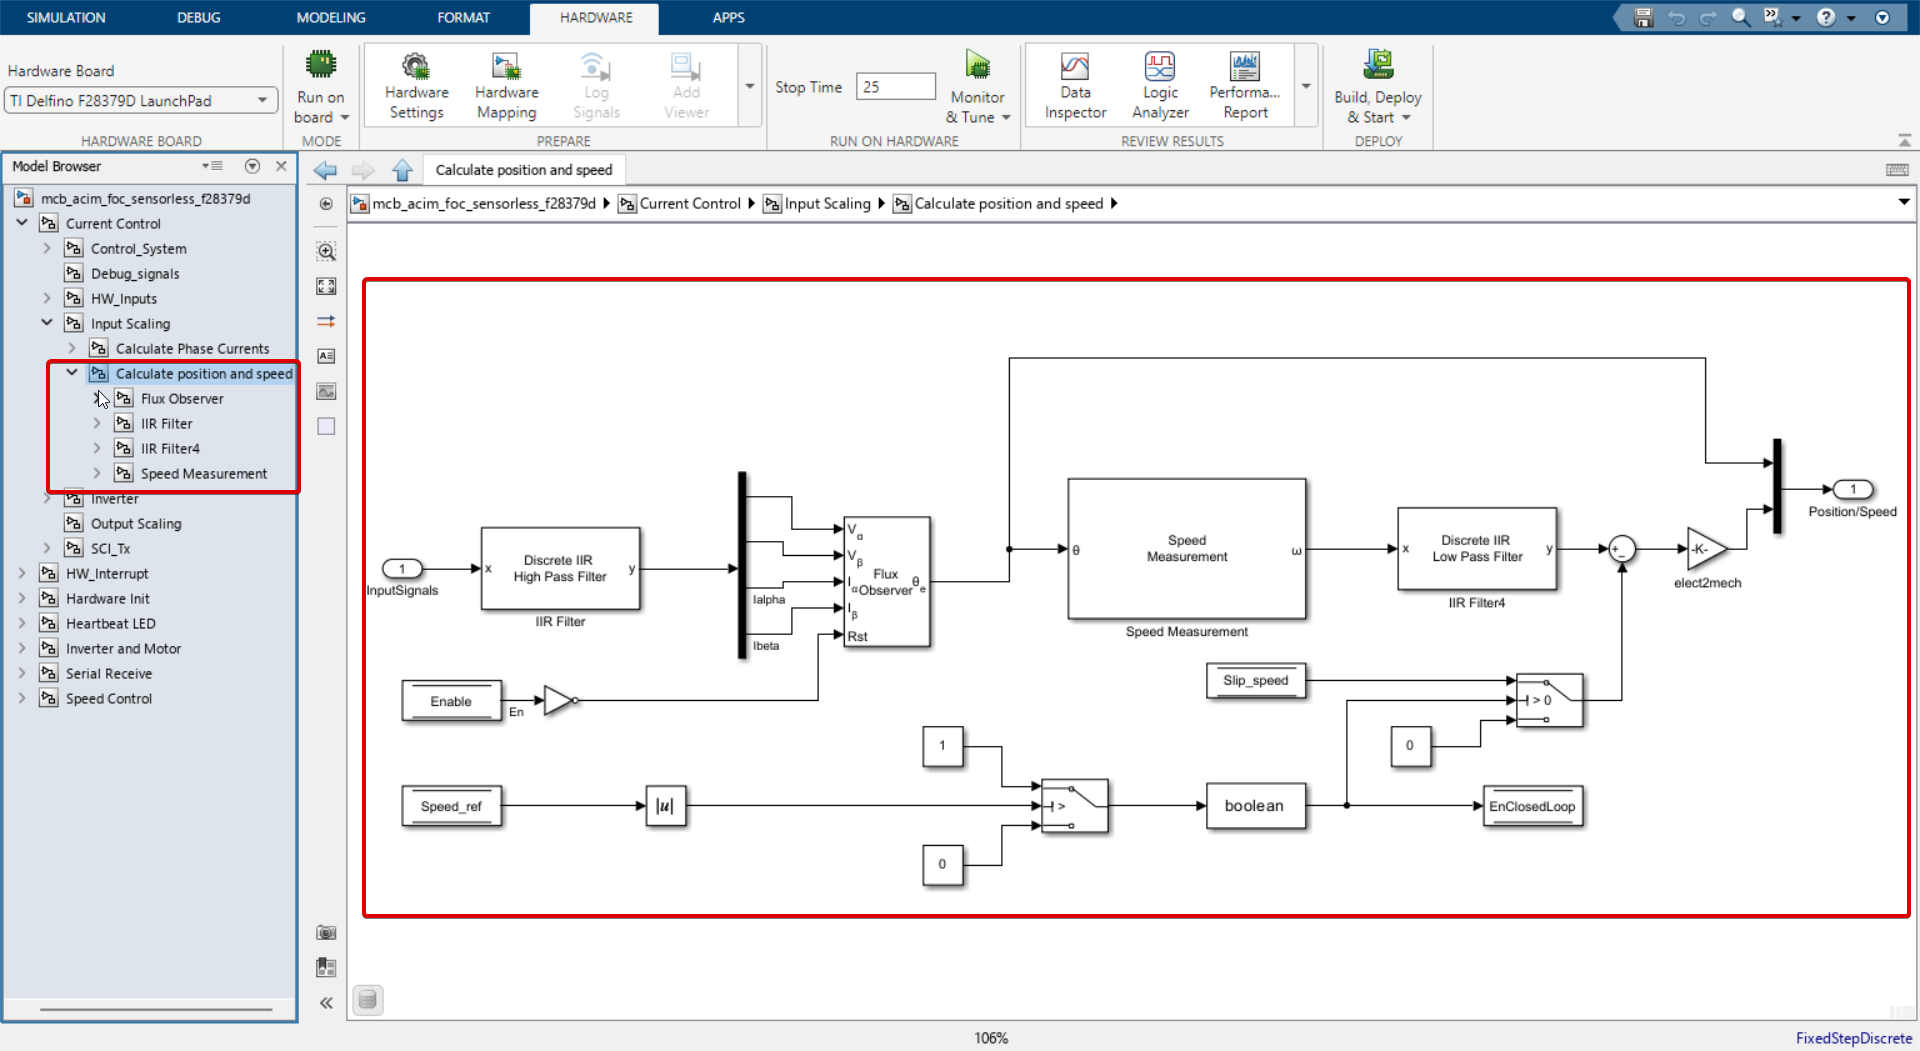
\includegraphics[width=4in]{sections/section3/images/simulation/inputScaling/fluxObserver.png}
	\caption{Position and Speed Estimation}
	\label{fig:position_speed_estimation}
\end{figure}


The position and speed estimation part of the Input Scaling block shown in  Figure \ref{fig:position_speed_estimation} uses the $VI_{fb}$ signal, which contains the motor's voltage and current in the $\alpha \beta$ reference frame. This signal goes through a high-pass filter to remove low-frequency noise. The filtered signals are then fed into the Flux Observer block, which estimates the stator flux position. The estimated stator flux position is then used in the Speed Estimation block to calculate the motor's speed. The estimated speed is filtered using a low-pass IIR filter to remove high-frequency noise. The final rotor speed is calculated by subtracting the slip speed from the estimated stator flux speed and then dividing by the number of pole pairs to get the mechanical speed.

\subsubsection{Control System}



\begin{figure}[H]
	\centering
	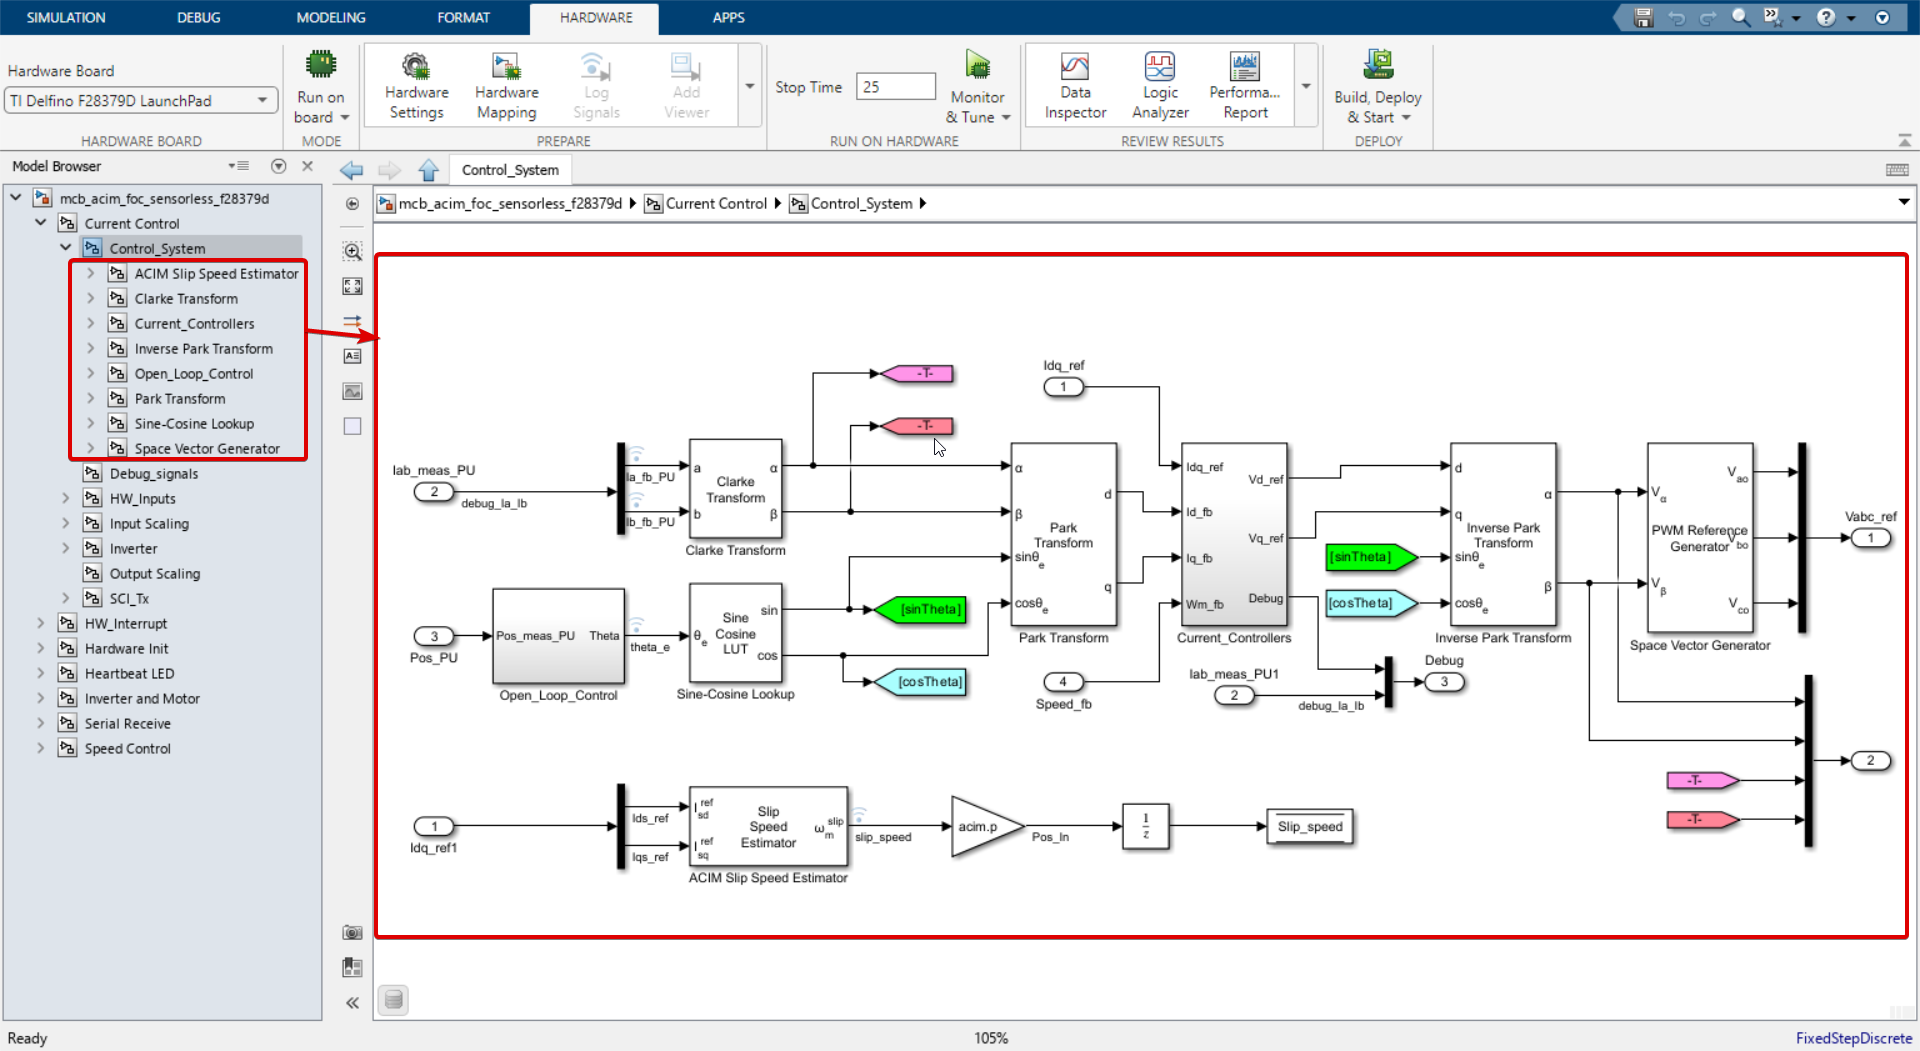
\includegraphics[width=4in]{sections/section3/images/simulation/currentControl/controlSystem.png}
	\caption{Current Control System}
	\label{fig:current_control_system}
\end{figure}


The control system shown in Figure \ref{fig:current_control_system} implemented in the inner current loop consists of two main components: the current controllers and the DQO transformation.

The current controllers use Proportional-Integral (PI) controllers to minimize the error between the reference currents ($I_{dq\_{ref}}$) and the feedback currents ($I_{d\_fb}$ and $I_{q\_fb}$). The output of the PI controllers is then limited, filtered, and adjusted using a feedforward controller and a saturation function to ensure safe and reliable operation of the system. The adjusted d-axis current is then used to generate the reference voltages ($V_{d\_{ref}}$ and $V_{q\_{ref}}$) in the DQ frame. These reference voltages are then transformed into the alpha-beta frame using the stator flux position ($\theta$) and fed into the PWM reference generator block, which generates the three-phase voltage references for the inverter. This inner current loop ensures that the actual currents closely follow the desired reference currents, which is crucial for the overall performance and stability of the control system.



\subsection{SIMULATION RESULTS}


\subsubsection{Load Angle}


\begin{figure}[H]
	\centering
	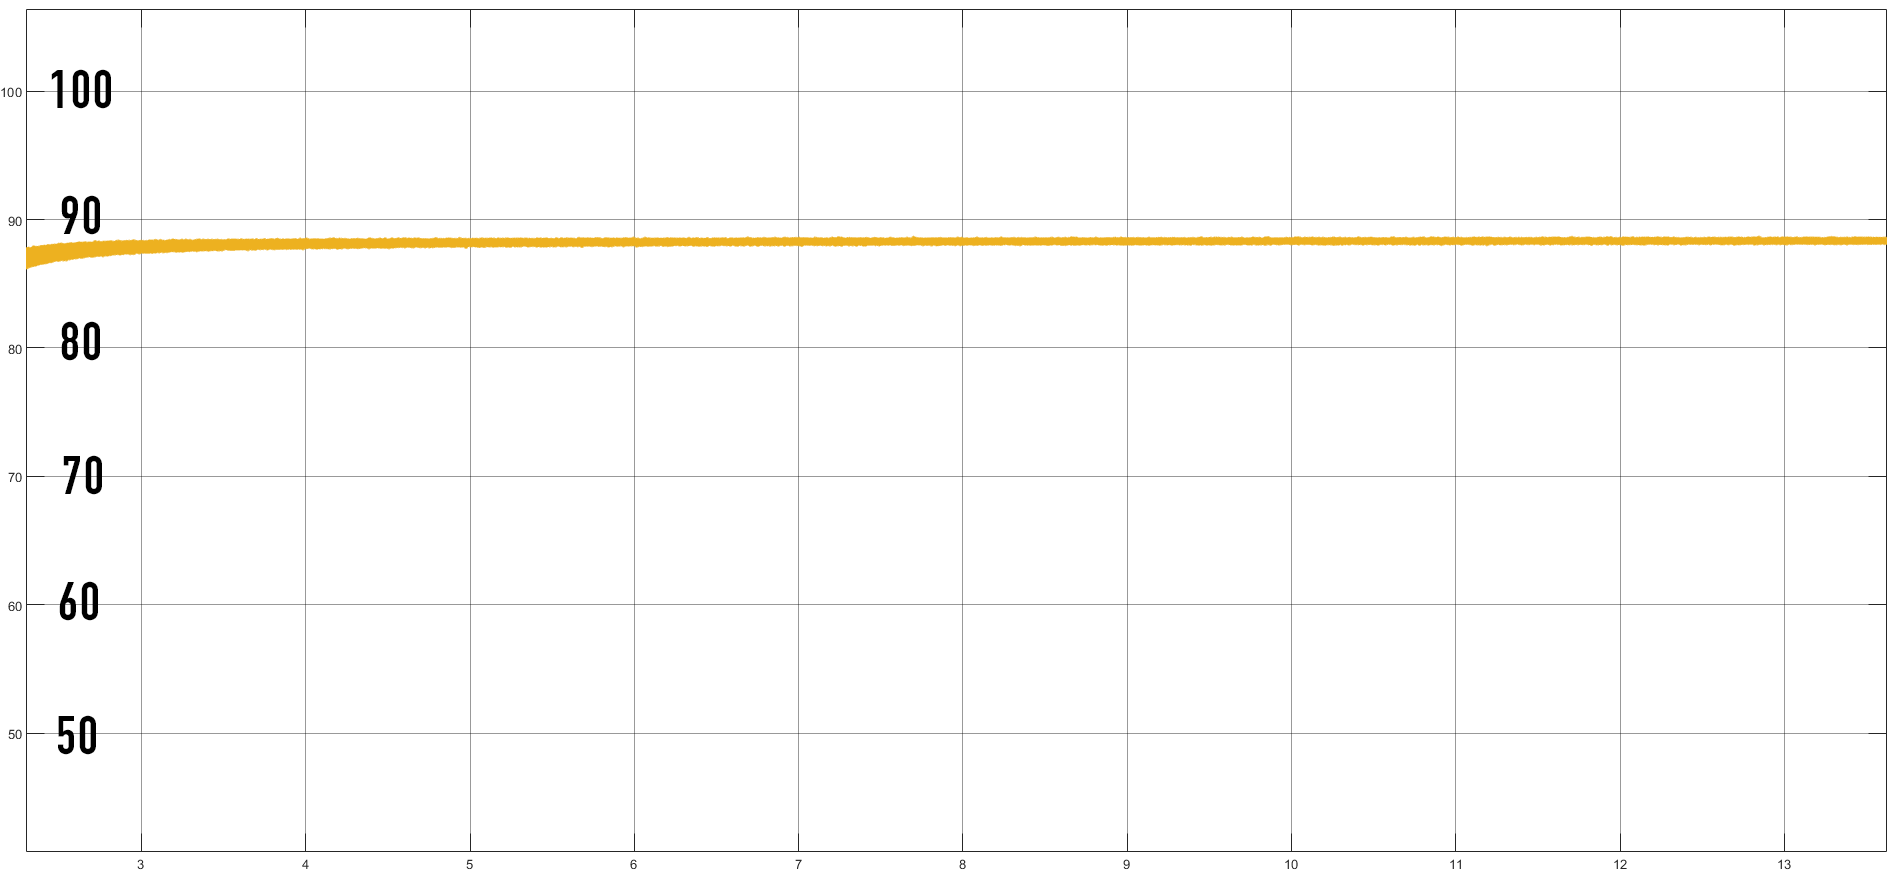
\includegraphics[width=6in]{sections/section3/images/simulationResutls/LoadAngle.png}
	\caption{Load Angle between Rotor Flux and Stator Flux}
	\label{fig:load_angle_1}
\end{figure}

Figure \ref{fig:load_angle_1} shows the load angle between the rotor flux and the stator flux. The x-axis indicates time (in seconds), and the y-axis denotes the load angle (in degrees). The waveform illustrates how the load angle changes over time, eventually settling around 90 degrees.

The load angle, also known as the torque angle, is a critical parameter in the vector control of induction machines. It is the angle between the rotor flux vector and the stator current vector in the rotor-flux-oriented reference frame. The load angle is directly related to the electromagnetic torque produced by the motor. 

In the ideal case of maximum torque per ampere control strategy, the load angle should be maintained at 90 degrees. This is because the torque produced by the induction machine is directly proportional to the sine of the load angle. Therefore, to maximize the torque output for a given current, the load angle should be maintained at 90 degrees, where the sine function reaches its maximum value.

The settling of the load angle around 90 degrees in the simulation results indicates that the vector control system is effectively controlling the motor to operate at the point of maximum efficiency. This validates the performance of the control system in managing the machine's dynamics and achieving efficient operation.


\begin{figure}[H]
	\centering
	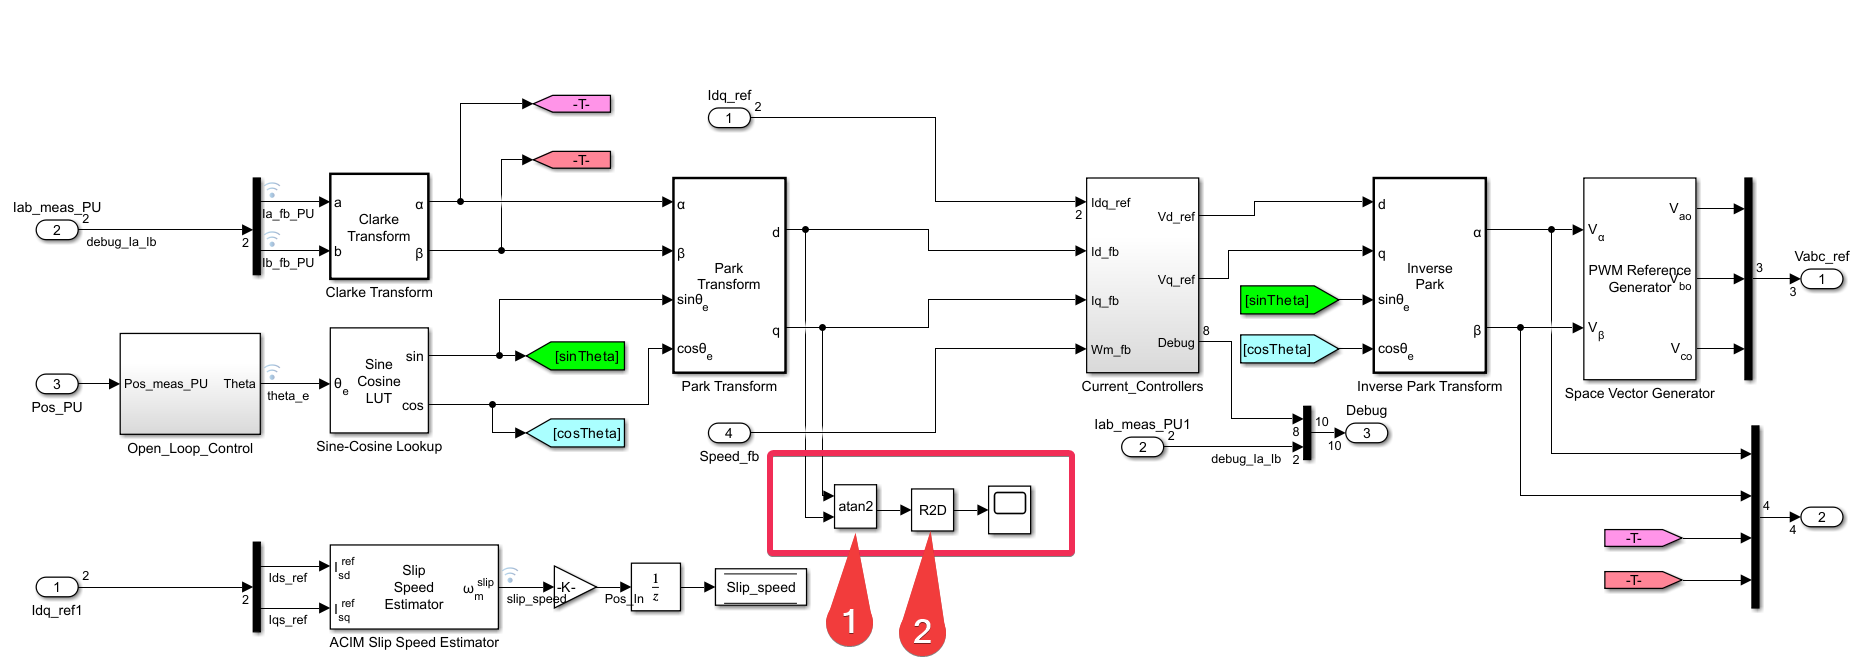
\includegraphics[width=6in]{sections/section3/images/simulationResutls/howTogetloadAngle.png}
	\caption{Simulink Model for Load Angle Calculation}
	\label{fig:loadAngleBlocks}
\end{figure}


Figure \ref{fig:loadAngleBlocks} shows the Simulink model and exact blocks used for getting the load angle. The model includes Park transform blocks, which are used to transform the three-phase stator currents into the rotor-flux-oriented reference frame. The transformed $D$ and $Q$ currents are then input to the `\texttt{Atan2}' block labeled 1 in the figure.

The `\texttt{Atan2}' block, also known as the four-quadrant inverse tangent function, calculates the angle from the $D$ and $Q$ currents. Unlike the standard inverse tangent function, the `\texttt{Atan2}' function takes two arguments and can return values in all four quadrants, which is necessary for accurately representing the load angle.

The output of the `\texttt{Atan2}' block, which is the load angle in radians, is then converted to degrees using the `\texttt{Radian to Degree}' block labeled 2 in the figure. The final output is displayed on a scope, which shows the load angle over time.




\subsubsection{Speed Response}

\begin{figure}[H]
	\centering
	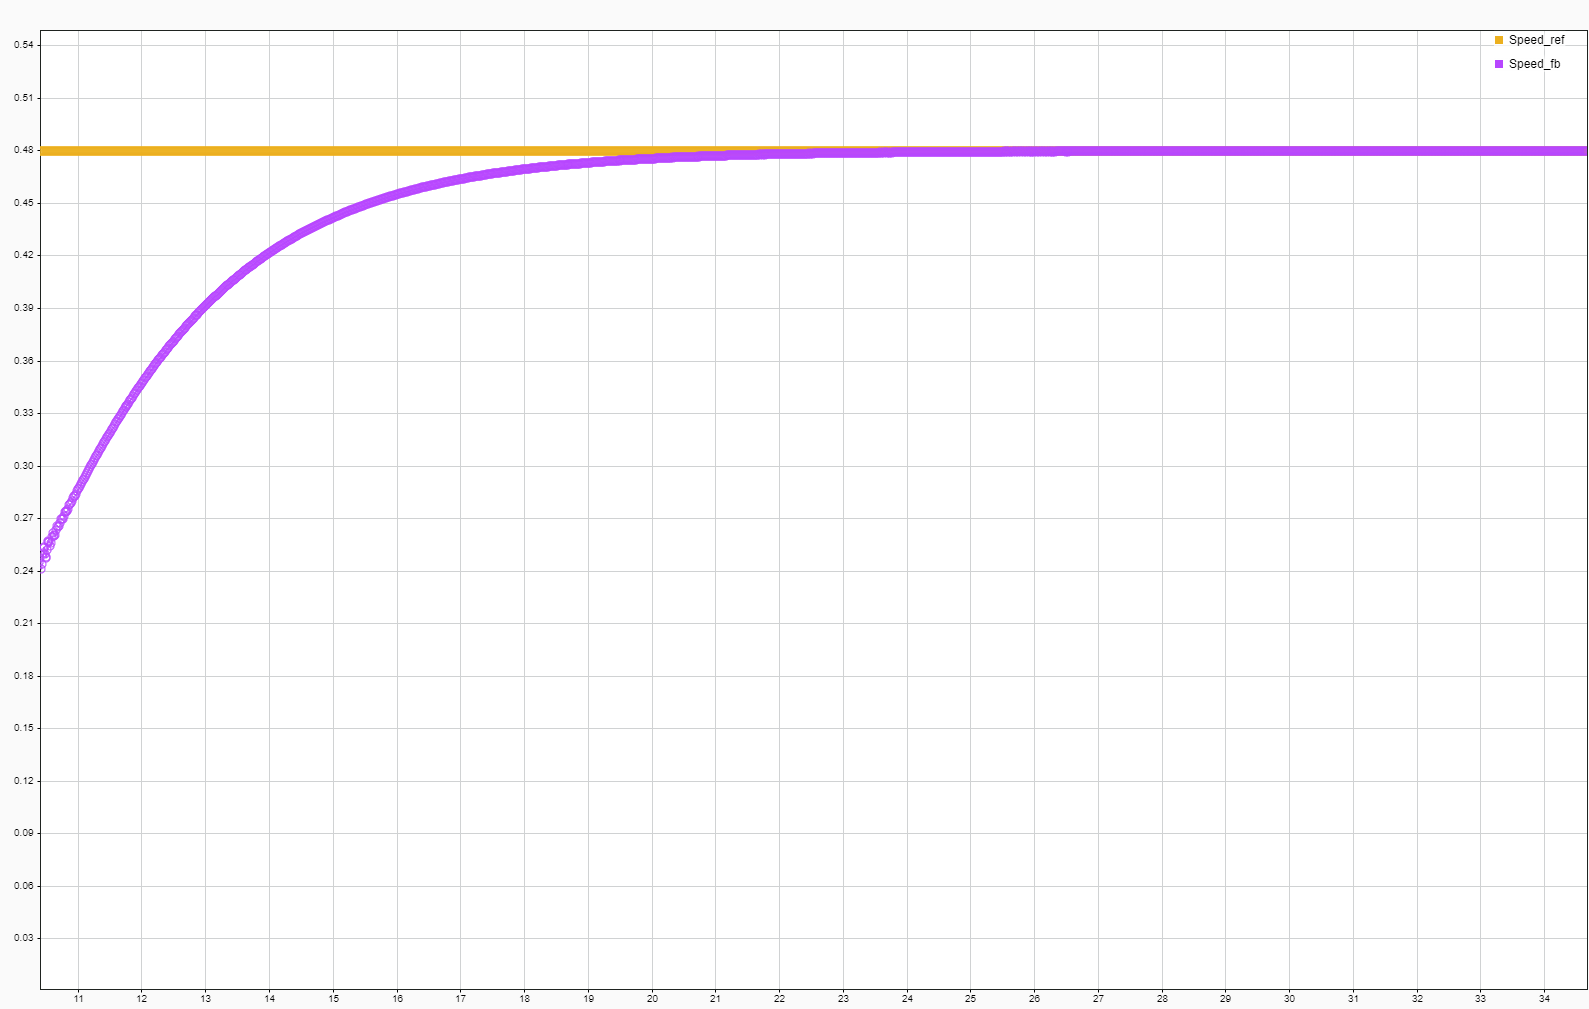
\includegraphics[width=6in]{sections/section3/images/simulationResutls/SpeedTrackingNoCursor.png}
	\caption{Speed Response}
	\label{fig:speed_response}
\end{figure}

Figure \ref{fig:speed_response} shows the speed response of the induction machine under vector control. The x-axis represents time (in seconds), and the y-axis represents speed (in RPM). The waveform demonstrates the machine's speed over time. The speed reference is set to 0.5 pu. The speed response shows that the machine's speed closely follows the reference, indicating the effectiveness of the speed control subsystem in managing the motor's speed.



\begin{figure}[H]
	\centering
	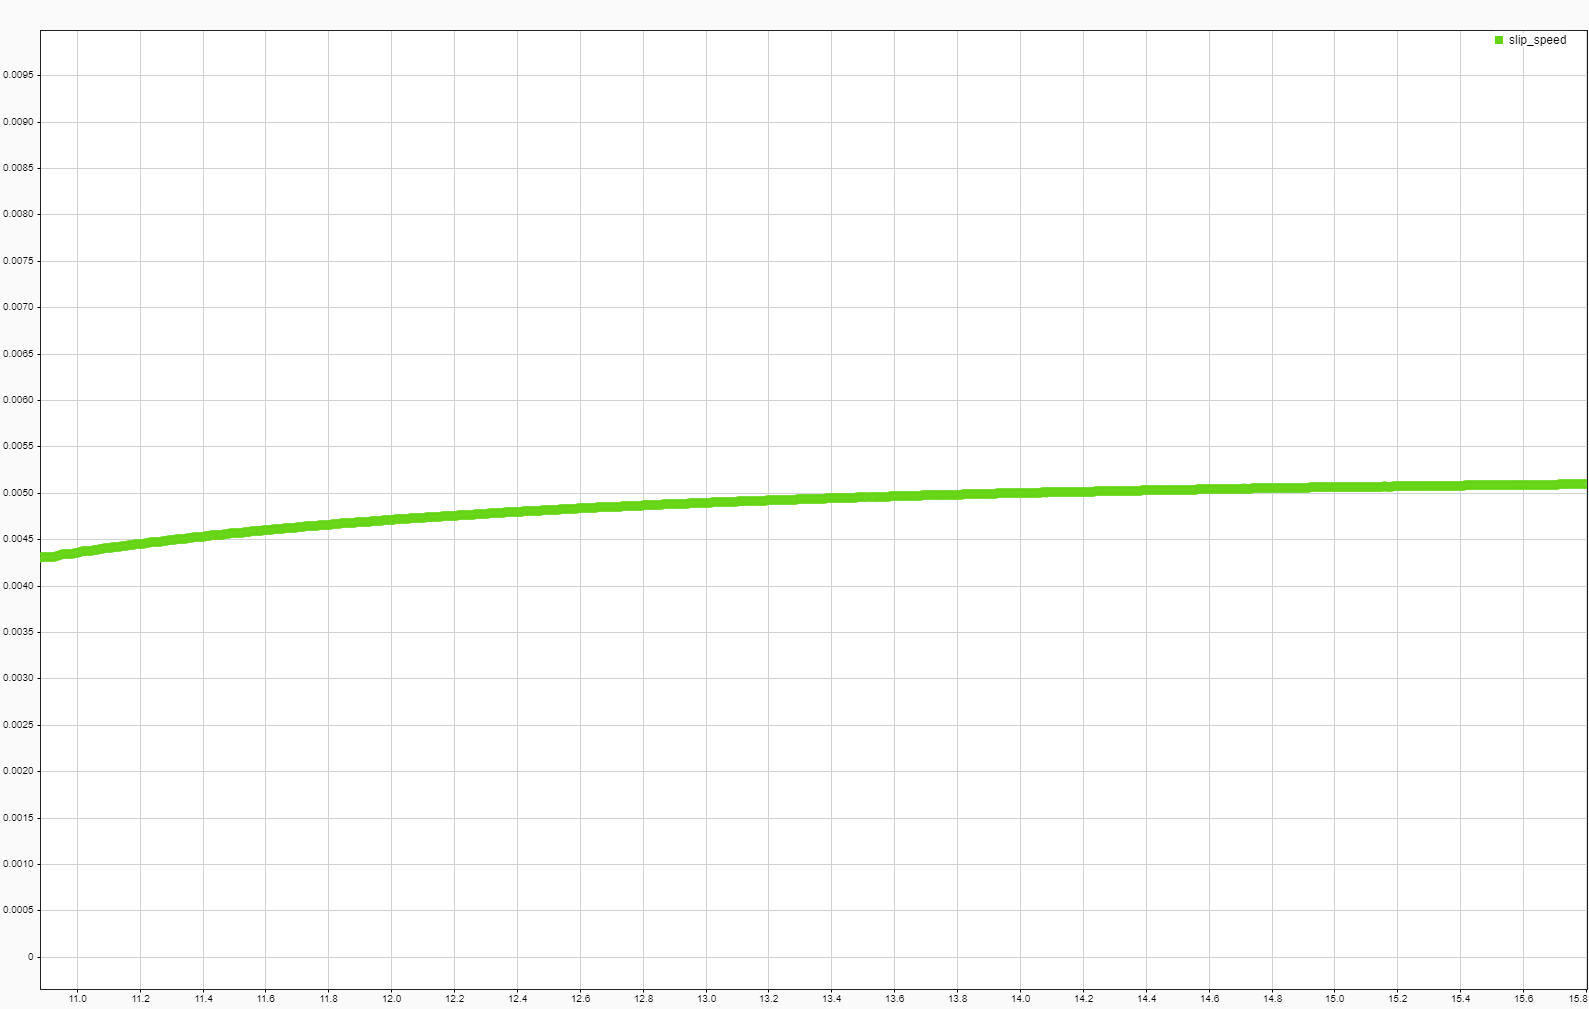
\includegraphics[width=6in]{sections/section3/images/simulationResutls/SlipSpeed.png}
	\caption{Slip Speed}
	\label{fig:slip_speed}
\end{figure}

Figure \ref{fig:slip_speed} represents the slip speed of the induction machine. The x-axis indicates time (in seconds), and the y-axis denotes the slip speed. The waveform illustrates how the slip speed changes over time. 





\subsubsection{Current Response}

Figure \ref{fig:current_response_IA_IB} displays the feedback or measured currents for Ia and Ib. The x-axis signifies time (in seconds), and the y-axis represents current (in per unit).

\begin{figure}[H]
	\centering
	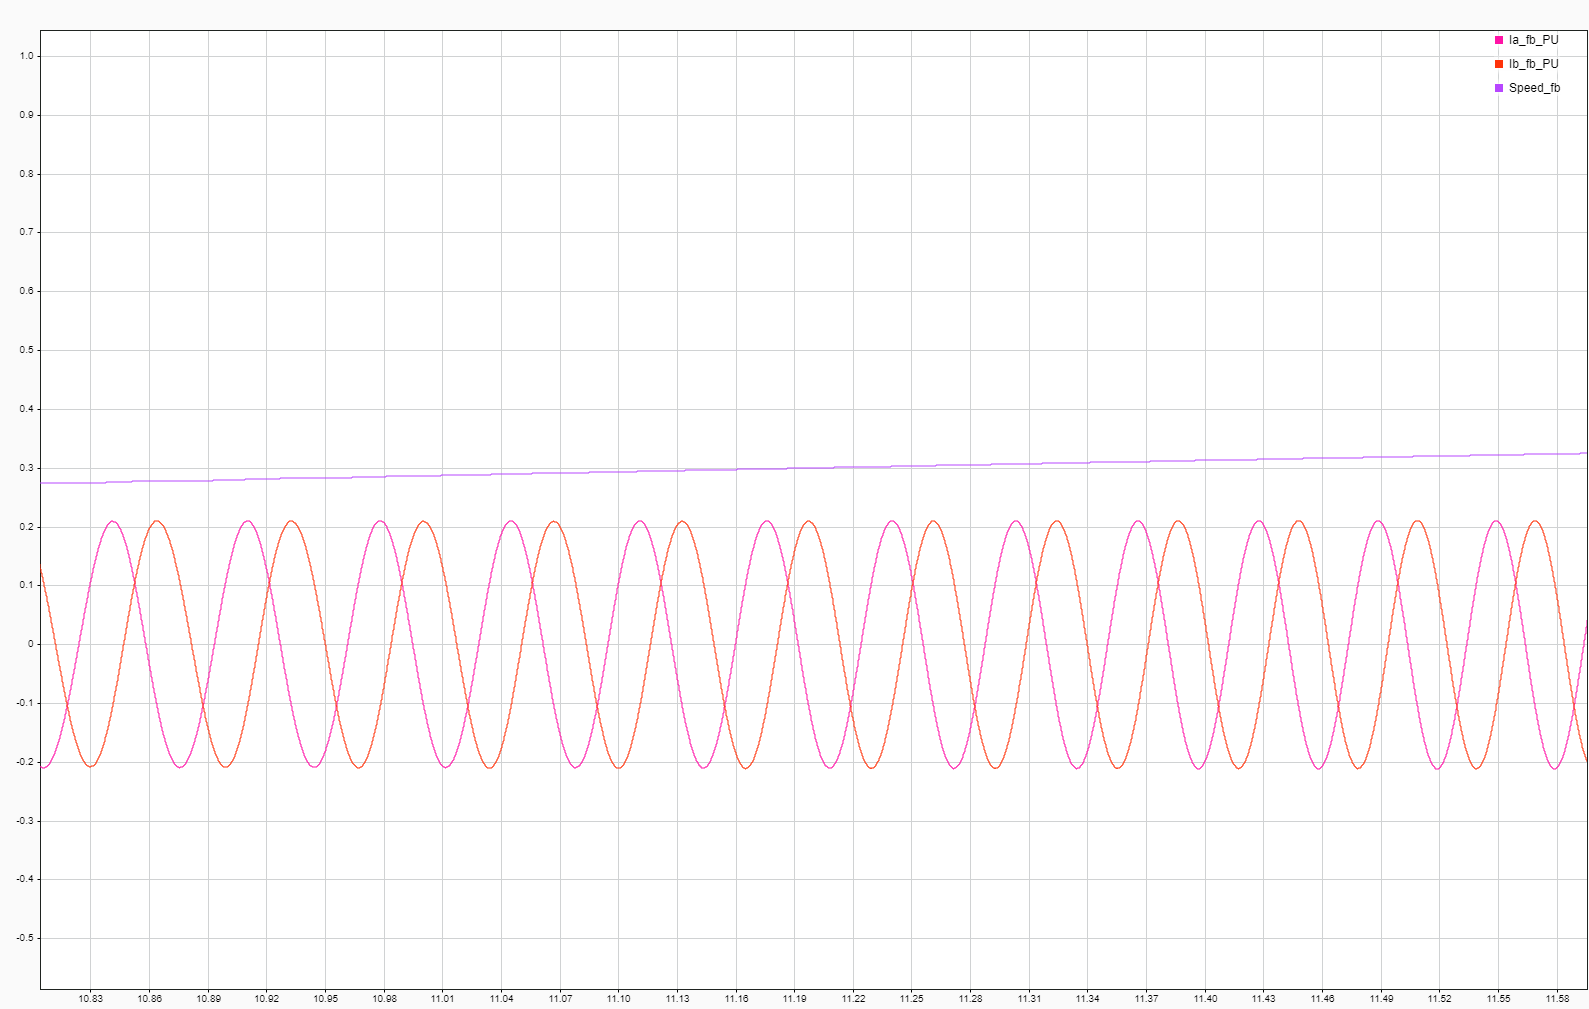
\includegraphics[width=6in]{sections/section3/images/simulationResutls/Ia_Ib_fb.png}
	\caption{Ia and Ib Feedback/Measured Currents}
	\label{fig:current_response_IA_IB}
\end{figure}



\begin{figure}[H]
	\centering
	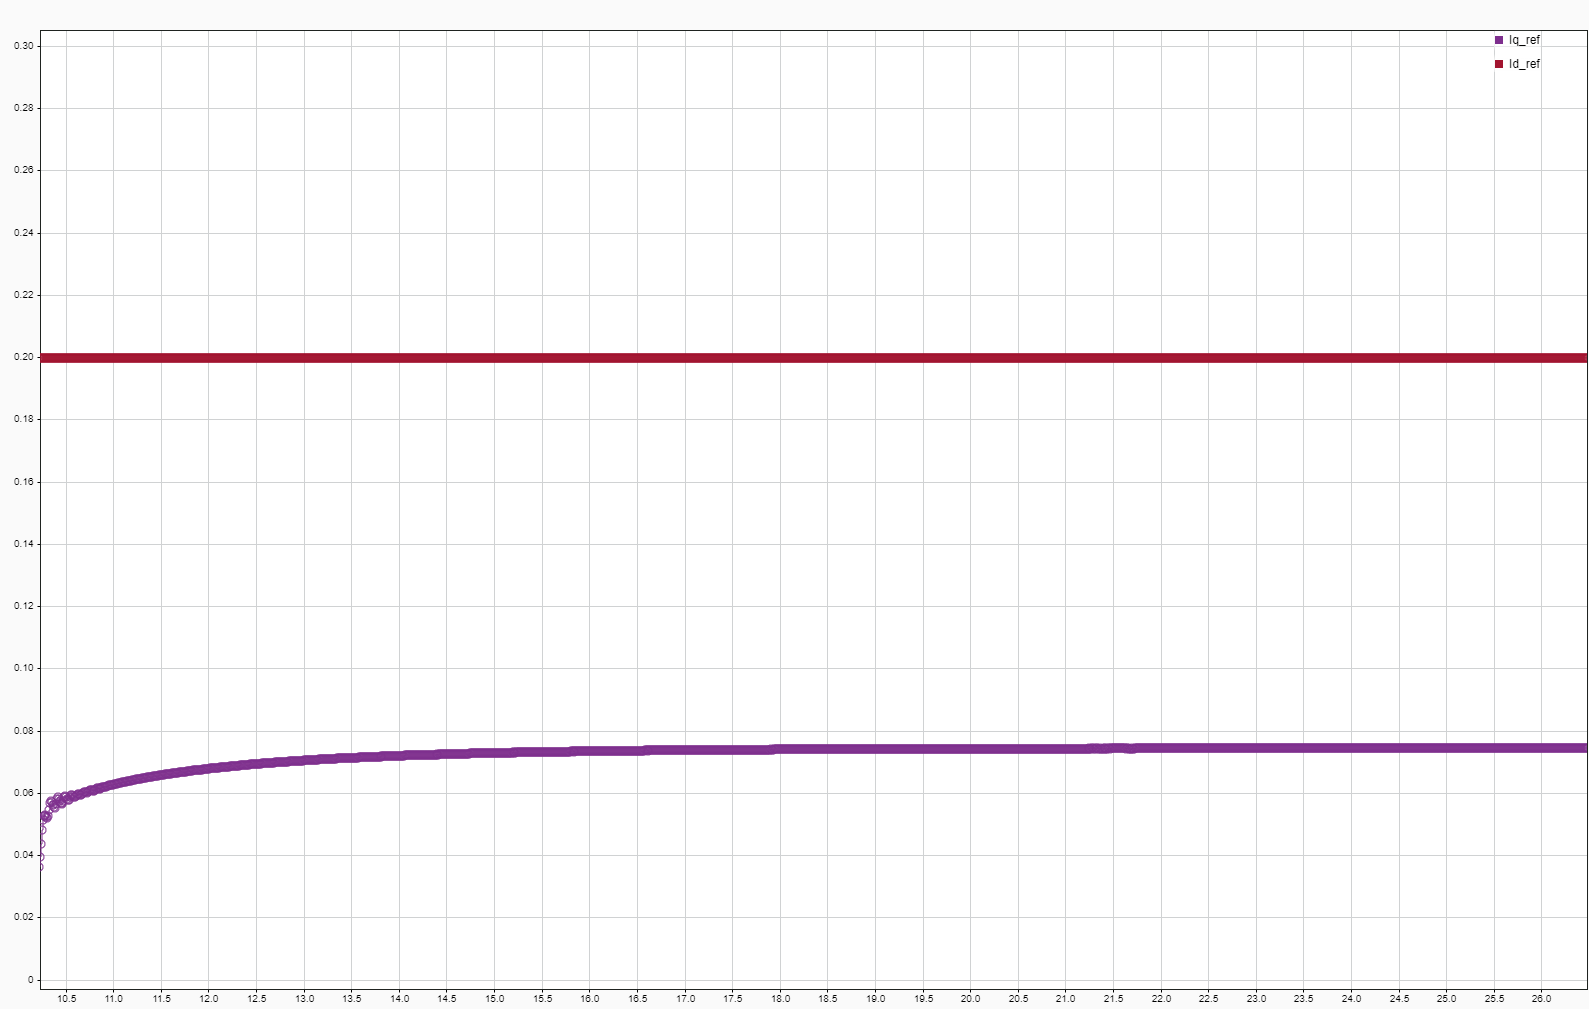
\includegraphics[width=6in]{sections/section3/images/simulationResutls/Id_ref_Iq_ref.png}
	\caption{Id and Iq Reference Currents}
	\label{fig:current_response_Id_ref_Iq_ref}
\end{figure}

The figure \ref{fig:current_response_Id_ref_Iq_ref} shows the reference currents for Id and Iq. The x-axis indicates time (in seconds), and the y-axis represents current (in per unit). The waveform illustrates how the reference currents change over time.


\begin{figure}[H]
	\centering
	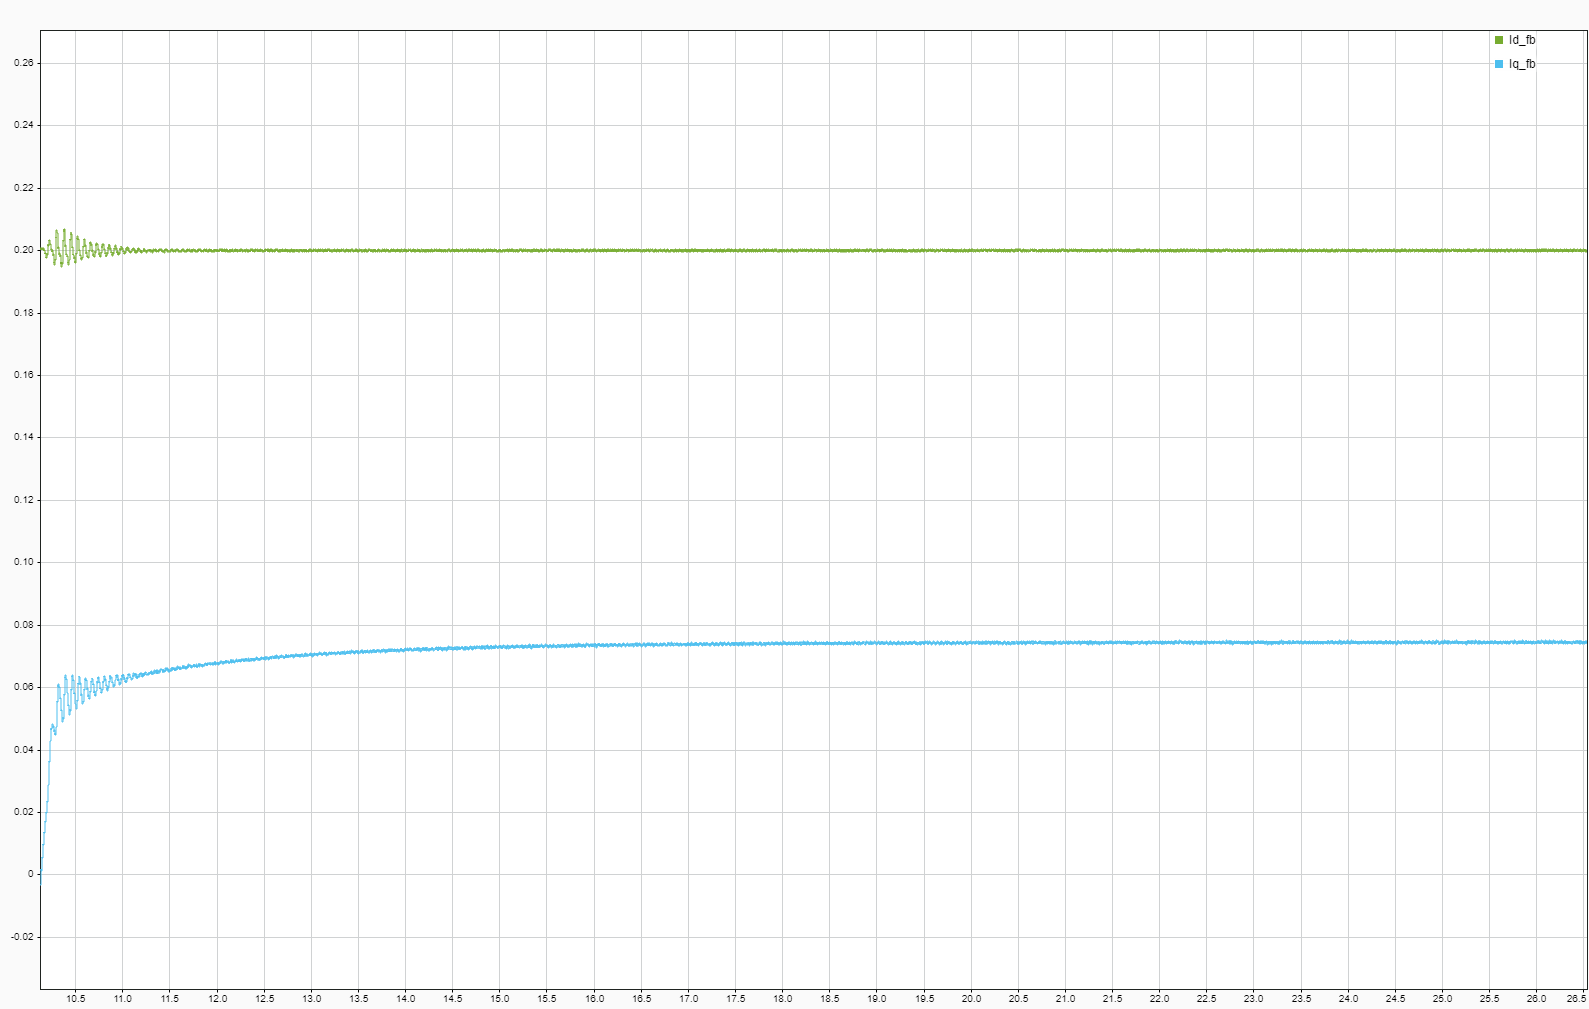
\includegraphics[width=6in]{sections/section3/images/simulationResutls/Id_fb_Iq_fb.png}
	\caption{Id and Iq Feedback Currents}
	\label{fig:current_response_Id_fb_Iq_fb}
\end{figure}


The figure \ref{fig:current_response_Id_fb_Iq_fb} displays feedback currents for Id and Iq. The x-axis represents time (in seconds), and the y-axis denotes current (in per unit). The waveform demonstrates the changes in the feedback currents over time. The observed trends can be attributed to load variations and control system responses.


The figure \ref{fig:current_response_Iq_ref_fb} shows the reference and feedback currents for Iq, which is responsible for producing torque. The x-axis signifies time (in seconds), and the y-axis represents current (in per unit). The waveform illustrates how these currents change over time. 

\begin{figure}[H]
	\centering
	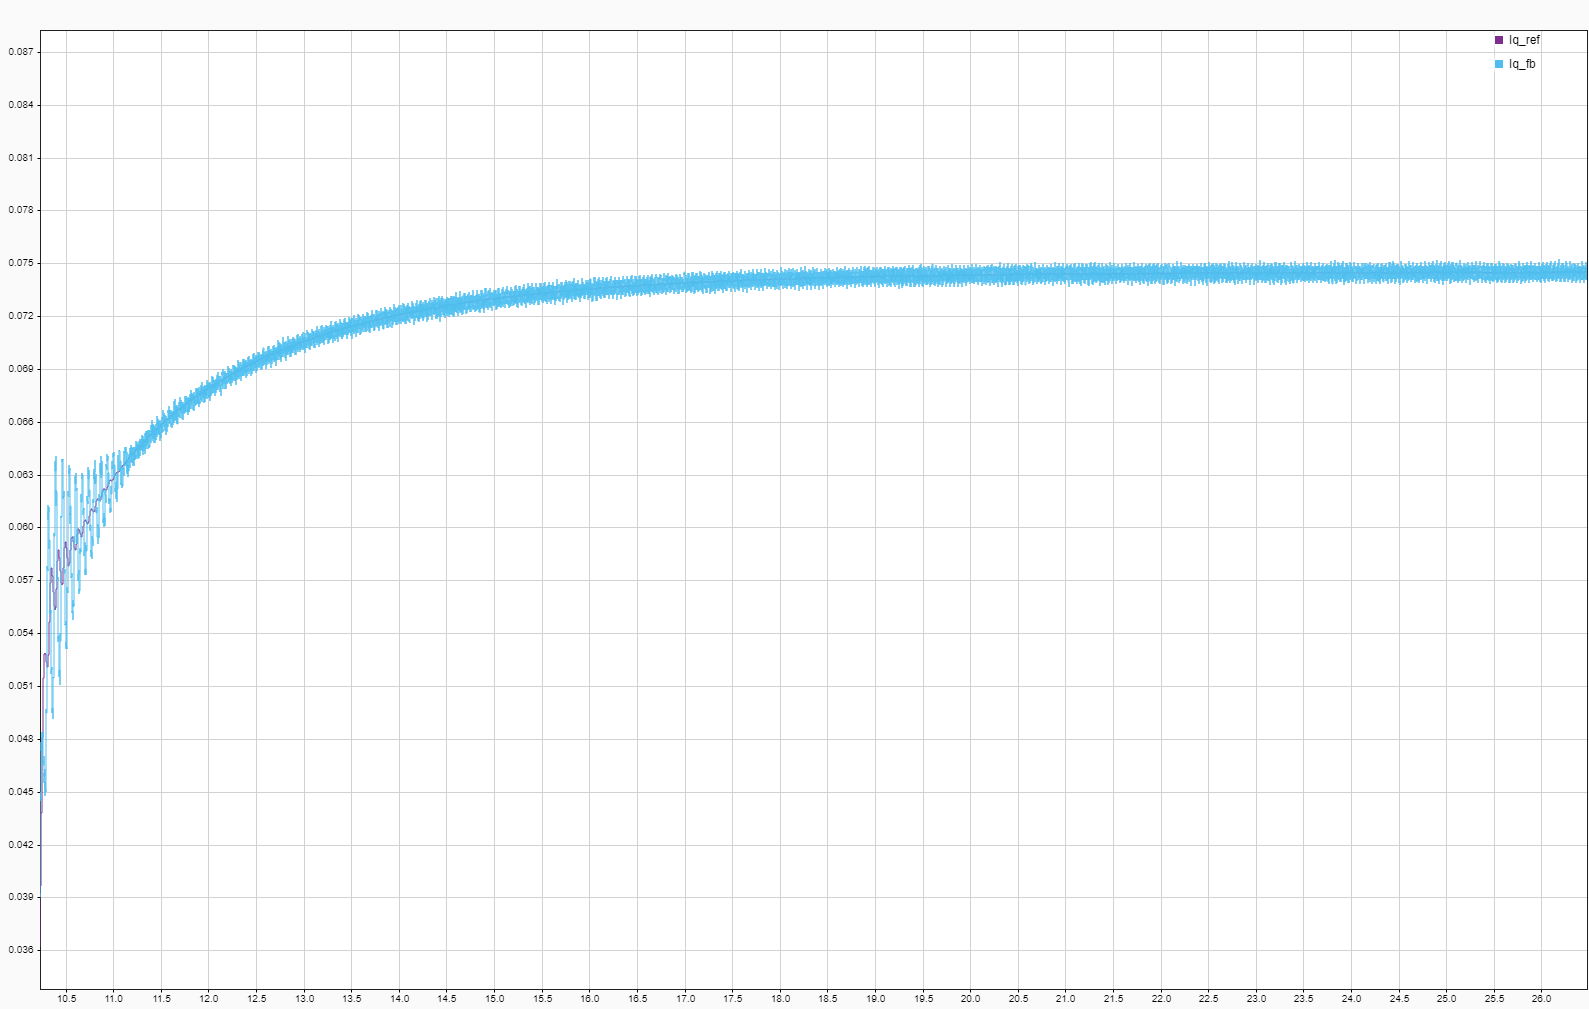
\includegraphics[width=6in]{sections/section3/images/simulationResutls/Iq_ref_fb.png}
	\caption{Iq Reference and Feedback Currents (Torque producing current)}
	\label{fig:current_response_Iq_ref_fb}
\end{figure}


The figure \ref{fig:current_response_Id_ref_fb}  displays the reference and feedback currents for Id, which is responsible for magnetizing the motor. The x-axis indicates time (in seconds), and the y-axis represents current (in per unit). The waveform illustrates how these currents change over time. The oscillations at the beginning of the simulation are due to the initial transient response of the control system as it tries to stabilize the motor currents.

\begin{figure}[H]
	\centering
	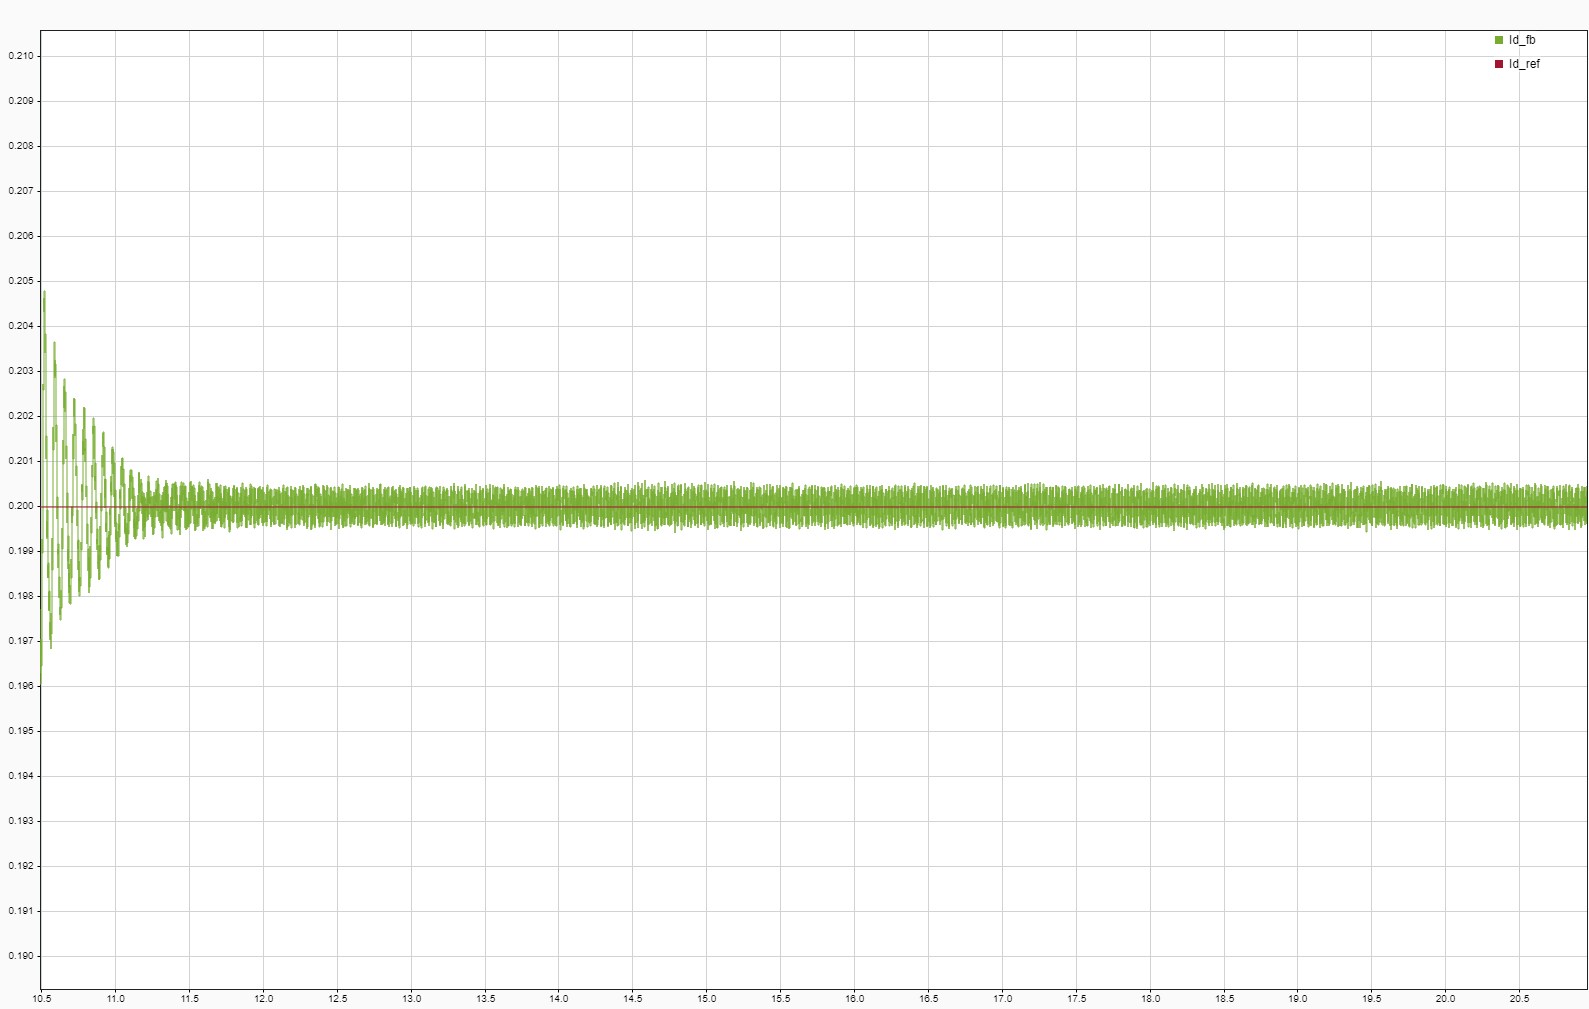
\includegraphics[width=6in]{sections/section3/images/simulationResutls/Id_ref_fb.png}
	\caption{Id Reference and Feedback Currents (Magnetizing current)}
	\label{fig:current_response_Id_ref_fb}
\end{figure}



\subsection{CHAPTER SUMMARY}

This chapter presented the simulation results FOC control system for an AC induction motor. The simulation was structured to validate various subsystems including speed control, current measurement, position and speed estimation, and the overall control system. Each section provided detailed insights through block diagrams and response graphs to illustrate the system's performance under simulated conditions.

\subsection{KEY FINDINGS}

\begin{itemize}
    \item The \textbf{Speed Control Subsystem} effectively managed the motor's speed by adjusting the torque reference values, ensuring that the motor speed follows the set reference closely.
    \item The \textbf{Current Control Subsystem} demonstrated robust performance in tracking the reference currents accurately, which is crucial for the stability and efficiency of the motor operation.
    \item \textbf{Position and Speed Estimation} techniques were validated to show precise estimation of the motor's speed and position, which are critical for the effective vector control of the AC induction motor.
    \item The overall system showed a \textbf{high degree of accuracy and responsiveness} in the speed and current responses, validating the effectiveness of the designed control strategies in managing the dynamics of the AC induction motor.
\end{itemize}

In conclusion, this chapter has laid a solid foundation for the practical implementation of the control system, with simulation results strongly supporting the theoretical designs.


\newpage